%-----------------------------------------------------------------------------------------------%
%
% Maret 2019
% Template Latex untuk Tugas Akhir Program Studi Sistem informasi ini
% dikembangkan oleh Inggih Permana (inggihjava@gmail.com)
%
% Template ini dikembangkan dari template yang dibuat oleh Andreas Febrian (Fasilkom UI 2003).
%
% Orang yang cerdas adalah orang yang paling banyak mengingat kematian.
%
%-----------------------------------------------------------------------------------------------%


%-----------------------------------------------------------------------------%
\chapter{\babTiga}
%-----------------------------------------------------------------------------%


%-----------------------------------------------------------------------------%
\section{Metode Pengembangan Sistem}

Pada metode ini akan membahas tetang metodologi penelitian yang dilakukan dalam penyusunan Tugas Akhir ini menggunakan metode \textit{Waterfall} meliputi \textit{User Requitmetns, System Requitments Analisis, Design}, Impelentasi, Sistem adapun dalam penelitian ini penulis membatasi tahapan penelitian hingga tahapan Implementasi sedangkan tahapan Sistem digantikan dengan tahapan Dokumentasi Laporan Tugas Akhir dapat dilihat pada \pic~\ref{gbr301}.


\begin{figure}
	\centering
	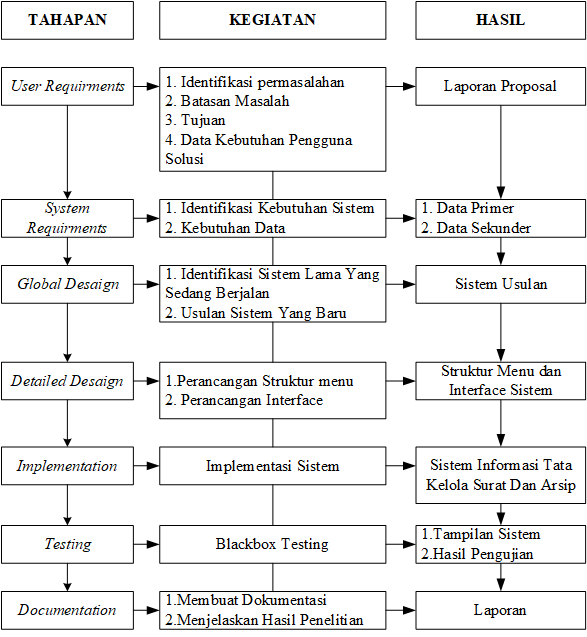
\includegraphics [height=8cm, width=10cm]{konten/gambar/gbr301.png}
		\caption{Metodologi Penelitian}
	\label{gbr301}
\end{figure}

\subsection{\textit{User Requitments}}
Tahap kebutuhan user merupakan tahap mengidentifikasi siapa saja user yang memiliki akses dan tugas masing-masing. Hal ini sangat penting karena kebutuhan pengguna atau user yang terlibat akan menggunakan sistem.

\subsection{\textit{System Requitments}}
Identifikasi Kebutuhan Sistem
Dalam analisa kenbutuhan sistem ada hal-hal yang di perhatikan untuk mengidentifikasi untuk perancangan sistem kedepannya. Hal-hal yang dilakukan pada tahap ini adalah :
Mengidentifikasi masalah alur sistem yang sedang berjalan Dinas Kesehatan Kabupaten Pelalawan dan penulis mewawancarai Kepala Bagian Umum Dinas Kesehatan Kabupaten Pelalawan. Pengambilan data yang dihasilkan dalam wawancara baik berupa data wawancara dan keterangan serta pernyataan narasumber.
\begin{enumerate}
	\item 	Data Primer
	\begin{enumerate}
		\item 	Observasi \\
		Pada tahap observasi ini untuk mengumpulkan informasi tentang lebih mengetahui permasalahan yang diteliti dan kondisi di lapangan (system requirements). Observasi dalam penelitian ini bertujuan untuk memperoleh gambaran mengenai objek penelitian di Dinas Dinas Kesehatan Kabupaten Pelalawan dengan pengambilan data yang dibutuhkan.
		\item 	Dokumen Surat\\
		Pengambilan data serta informasi tata naskah dinas pada Dinas Kesehatan Kabupaten Pelalawan.
		\item	Studi Pustaka\\
		Untuk menambah referensi, penulis melakukan studi pustaka dengan mencari referensi yang terkait dengan topik penelitian tugas akhir ini. Sumber yang penulis gunakan adalah buku-buku dan jurnal yang berkaitan dengan topik penelitian serta data sekunder yang didapat dari Dinas Kesehatan Kabupaten Pelalawan.
	\end{enumerate}
	
	\item Data Sekunder \\
	Data sekunder yaitu data yang diperoleh secara tidak langsung atau data yang diperoleh selain dari objek penelitian. Dalam penelitian ini sumber data sekunder yang digunakan berbentuk data file baik foto dan ddokumen yang di dapat langsung dari Dinas Kesehatan Kabupaten Pelalawan dapat dilihat pada Lampiran A 

\end{enumerate}


\subsection{Global Design}
Pada tahap ini merupakan melakukan perancangan sistem yang di usulkan. Tahap Global Design merupakan tahap dalam perancangan sistem yang akan dibangun berdasarkan analisis sistem yang sebelumnya telah dilaksanakan.
\begin{enumerate}
	\item 	Alur Sistem Lama.\\
	Mengetahui alur sistem yang sedang berjalan sebelumnya adalah sebuah langka untuk merancangan sistem usulan yang akan di buat oleh peneliti. Analisis sistem yang sedang berjalan meruapakan analasis sistem yang dilakukan yaitu menganalisa sistem yang saat ini berjalan pada Dinas Kesehatan Kabupaten Pelalawan untuk mengidentifikasi permasalahan-permasalahan yang muncul.
	\item	Perancangan Sistem Usulan\\
	Perancangan sistem usulan adalah sebuah perancangan yang di rancang untuk mengtasi atau meminimalisir permasalahan yang ada pada sistem sebelumnya, adapun langkahnya, yaitu:
	\begin{enumerate}
		\item	Analisa Sistem Usulan\\
		Menganalisa permasalahan yang telah diidentifikasi untuk kemudian digunakan dalam dasar perancangan sistem sebagai solusi dari masalah dan memberikan rekomendasi manfaat sesuai kebutuhan dari instansi terkait. Perancangan alur yang akan dibangun dalam membangun system informasi pariwisataDinas Kesehatan Kabupaten Pelalawan adalah merancang bagaimana alur atau jalannya sistem yang akan dibangun berdasarkan wawancara terhadap pihakDinas Kesehatan Kabupaten Pelalawan dan peranan aktor yang terlibat dalam proses sistem. Perancangan alur sistem yang akan dibangun dirangkum dan di jelaskan pada BAB IV “Analisa dan Perancangan”.
		\item	Identifikasi Kebutuhan Sistem\\
		Tahapan ini berguna untuk mengidentifikasi dan menentukan kebutuan sistem yang akan di usulkan.
	\end{enumerate}
\end{enumerate}

\subsection{\textit{Design Detailed}}
Pada tahap ini perancangan yang di jelaskan lebih spesifik tetang perancangan sistem, adapun perancangannya, yaitu:
\begin{enumerate}
	\item 	Perancangan Struktur Menu\\
	Pada perancangan struktur menu terdapat  menu pada sistem yang akan dibangun. Perancangan struktur menu dibuat berdasarkan alur sistem yang telah dibangun sebelumnya. Struktur menu yang akan dirancang dibuat menggunakan tool Microsoft Visio 2019 yang dirangkum dalam BAB IV “Analisa dan Perancangan”.
	\item	Perancangan Interface\\
	Perancangan interface sistem bagaimana tampilan dari sistem yang akan dibangun peneliti. Interface tersebut didesain berdasarkan alur serta struktur menu yang telah dirancang sebelumnya. Interface sistem ini dibuat menggunakan tool Mockups Balsamic 3 yang terangkum dalam BAB IV “Analisa dan Perancangan”.
	\item	Perancangan sistem menggunakan UML dengan 4 (empat) Diagram yaitu, \textit{Use Case Diagram, Sequence Diagram, Class Diagram dan Activity Diagram}.
\end{enumerate}

\subsection{\textit{Implementation}}
Tahap Implementasi merupakan bagian pembuatan kode-kode program yang dibuat berdasarkan seluruh rancangan yang telah dibuat sebelumnya untuk proses selanjutnya, pengolahan data dan pembuatan sistem informasi tatakelola surat dan arsip. Kegiatan dari tahap implementasi meliputi:
\begin{enumerate}
	\item 	Pengolahan Data\\
	Pengolahan data spasial menggunakan database MySQL, dengan server Apache Server, framework Codeigniter dan bootsraap sebagai tampilan interface.
	\item 	Pembuatan kode-kode program atau coding menggunakan Bahasa pemograman PHP.
	\item 	Pada tahap pengkodingan ini dilakukan setelah data yang dibutuhkan terkumpul dan telah diolah sesuai kebutuhan untuk merancang sistem informasi tatakelola surat dan arsip di Dinas kesehatan Kabupaten pelalawan.
\end{enumerate}

\subsection{\textit{Testing}}
Tahap pengujian adalah  tahap yang dilakukan adalah melakukan pengujian menggunakan Blackbox testing yang merupakan pendekatan pengujian dengan mempelajari input dan output yang diberikan.Tahapan pengujian ini di lakukan dengan tujuan untuk menjamin sistem yang dibuat sesuai dengan hasil analisis dan perancangan serta menghasilkan satu kesimpulan apakah sistem tersebut sesuai dengan yang di harapkan.

\subsection{\textit{Documentation}}
Pada tahap ini yang dilakukan adalah melakukan dokumentasi dari semua tahap yang telah dilakukan. Mulai dari proses pendahuluan, perencanaan, pengumpulan data, analisis dan perancangan sistem, implementasi serta pengujian sistem. Kemudian mempresentasikan hasil penelitian dan menampilkan hasil sistem yang telah dibangun. Hasil dari dokumentasi ini adalah laporan Tugas Akhir.
